\section{Simulointi ja testaus}
Tässä kandidaattityössä käytettiin Matlab-ohjelmaa simuloimaan MUSIC-algoritmia ja sen eri versioita. Simulaatioita tehtiin yksinkertaisella pallomallilla sekä todellisten aivojen tilavuusjohdemallilla. Oikeiden aivojen päämalliverkot ja niiden johtokenttämatriisit on saatu Sara Sommarivalta. Mittausdatana käytettiin MEG-dataa, joka on saatu Johanna Metsomaalta. Apufunktiot pallomallilla simulointiin on saatu Jukka Sarvakselta. Koodit päämalliverkon mallinnukseen on saatu Matti Stenroosilta.

RAP- ja TRAP-MUSIC:lla yritettiin selvittää, kuinka monta lähdettä ne löytävät simuloidusta datasta. Simuloinneissa lähteiden määrän arvioitiin olevan siinä kohtaan, jossa vierekkäisten singulaariarvojen erotus on suurin.

Pallomallissa pään osat mallinnetaan kolmena johdepallona. Uloin pallo kuvaa päänahkaa, seuraava kalloa ja sisin pallo aivoja ja sen pinta aivokuorta. Jokaisella pallolla on homogeeninen johtavuus. Pallomallissa käytetyt johtavuudet ja säteet ovat merkittyinä alla oleviin taulukoihin \ref{table:johtavuus} ja \ref{table:sateet}.

\begin{table}[h]
\begin{minipage}{0.5\textwidth}
    \caption{Johtavuudet}
    \begin{center}
        \begin{tabular}{|c|c|}
            \hline
            & Johtavuudet ($\frac{1}{\Omega m}$)\\ \hline
            Päänahka & 0,33 \\
            Kallo & 0,0042 \\
            Aivot & 0,33 \\
            \hline
        
        \end{tabular}
    \end{center}
    \label{table:johtavuus}
\end{minipage}
\begin{minipage}{0.5\textwidth}
    \caption{Säteet}
    \begin{center}
        \begin{tabular}{|c|c|}
            \hline
            & Säteet (mm)\\ \hline
            Päänahka & 88 \\
            Kallon ulkopinta & 85 \\
            Kallon sisäpinta & 81 \\
            Aivokuori & 76 \\
            \hline
        \end{tabular}
    \end{center}
    \label{table:sateet}
\end{minipage}
\end{table}

Pallomallissa oletetaan, että lähteet sijaitsevat aivokuorella. Elektrodit sijoitetaan uloimman pallokuoren ja lähdedipolit sisimmän pallokuoren pinnalle. Lähdepisteet voidaan projisoida tasoon yksikköympyrälle ja MUSIC-algoritmin avulla muodostetaan kuva paikannusfunktion arvoista topografiana.

\begin{figure}[hb]
    \begin{minipage}{0.5\textwidth}
        \centering
        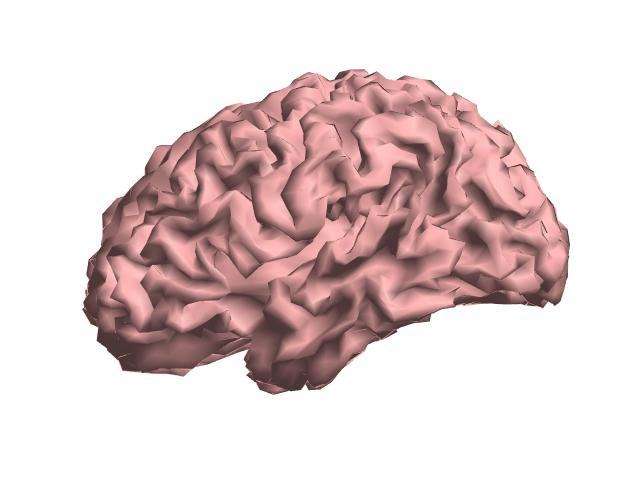
\includegraphics[width=0.9\textwidth]{aivot2.jpg}
    \end{minipage}
    \begin{minipage}{0.5\textwidth}
        \centering
        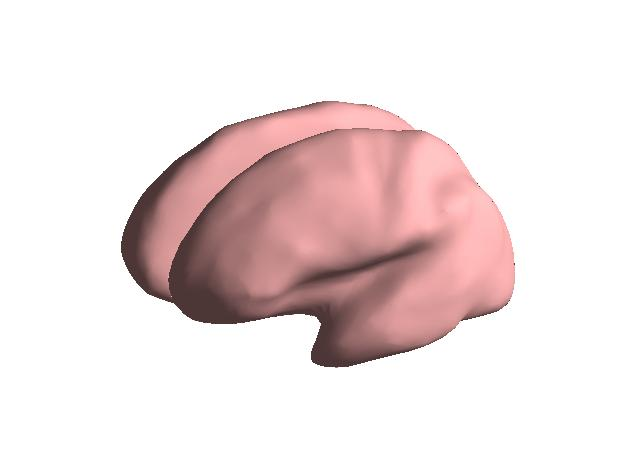
\includegraphics[width=\textwidth]{aivot.jpg}
    \end{minipage}
    \caption{Vasemmalla malli aivoista ja oikealla uurteet puhallettuna auki.}
    \label{fig:aivot}
\end{figure}
